% !TeX program = pdfLaTeX
\documentclass[12pt]{article}
\usepackage{amsmath}
\usepackage{graphicx,psfrag,epsf}
\usepackage{enumerate}
\usepackage{natbib}
\usepackage{textcomp}
\usepackage[hyphens]{url} % not crucial - just used below for the URL
\usepackage{hyperref}
\providecommand{\tightlist}{%
  \setlength{\itemsep}{0pt}\setlength{\parskip}{0pt}}

%\pdfminorversion=4
% NOTE: To produce blinded version, replace "0" with "1" below.
\newcommand{\blind}{0}

% DON'T change margins - should be 1 inch all around.
\addtolength{\oddsidemargin}{-.5in}%
\addtolength{\evensidemargin}{-.5in}%
\addtolength{\textwidth}{1in}%
\addtolength{\textheight}{1.3in}%
\addtolength{\topmargin}{-.8in}%

%% load any required packages here


\usepackage{color}
\usepackage{fancyvrb}
\newcommand{\VerbBar}{|}
\newcommand{\VERB}{\Verb[commandchars=\\\{\}]}
\DefineVerbatimEnvironment{Highlighting}{Verbatim}{commandchars=\\\{\}}
% Add ',fontsize=\small' for more characters per line
\usepackage{framed}
\definecolor{shadecolor}{RGB}{248,248,248}
\newenvironment{Shaded}{\begin{snugshade}}{\end{snugshade}}
\newcommand{\AlertTok}[1]{\textcolor[rgb]{0.94,0.16,0.16}{#1}}
\newcommand{\AnnotationTok}[1]{\textcolor[rgb]{0.56,0.35,0.01}{\textbf{\textit{#1}}}}
\newcommand{\AttributeTok}[1]{\textcolor[rgb]{0.77,0.63,0.00}{#1}}
\newcommand{\BaseNTok}[1]{\textcolor[rgb]{0.00,0.00,0.81}{#1}}
\newcommand{\BuiltInTok}[1]{#1}
\newcommand{\CharTok}[1]{\textcolor[rgb]{0.31,0.60,0.02}{#1}}
\newcommand{\CommentTok}[1]{\textcolor[rgb]{0.56,0.35,0.01}{\textit{#1}}}
\newcommand{\CommentVarTok}[1]{\textcolor[rgb]{0.56,0.35,0.01}{\textbf{\textit{#1}}}}
\newcommand{\ConstantTok}[1]{\textcolor[rgb]{0.00,0.00,0.00}{#1}}
\newcommand{\ControlFlowTok}[1]{\textcolor[rgb]{0.13,0.29,0.53}{\textbf{#1}}}
\newcommand{\DataTypeTok}[1]{\textcolor[rgb]{0.13,0.29,0.53}{#1}}
\newcommand{\DecValTok}[1]{\textcolor[rgb]{0.00,0.00,0.81}{#1}}
\newcommand{\DocumentationTok}[1]{\textcolor[rgb]{0.56,0.35,0.01}{\textbf{\textit{#1}}}}
\newcommand{\ErrorTok}[1]{\textcolor[rgb]{0.64,0.00,0.00}{\textbf{#1}}}
\newcommand{\ExtensionTok}[1]{#1}
\newcommand{\FloatTok}[1]{\textcolor[rgb]{0.00,0.00,0.81}{#1}}
\newcommand{\FunctionTok}[1]{\textcolor[rgb]{0.00,0.00,0.00}{#1}}
\newcommand{\ImportTok}[1]{#1}
\newcommand{\InformationTok}[1]{\textcolor[rgb]{0.56,0.35,0.01}{\textbf{\textit{#1}}}}
\newcommand{\KeywordTok}[1]{\textcolor[rgb]{0.13,0.29,0.53}{\textbf{#1}}}
\newcommand{\NormalTok}[1]{#1}
\newcommand{\OperatorTok}[1]{\textcolor[rgb]{0.81,0.36,0.00}{\textbf{#1}}}
\newcommand{\OtherTok}[1]{\textcolor[rgb]{0.56,0.35,0.01}{#1}}
\newcommand{\PreprocessorTok}[1]{\textcolor[rgb]{0.56,0.35,0.01}{\textit{#1}}}
\newcommand{\RegionMarkerTok}[1]{#1}
\newcommand{\SpecialCharTok}[1]{\textcolor[rgb]{0.00,0.00,0.00}{#1}}
\newcommand{\SpecialStringTok}[1]{\textcolor[rgb]{0.31,0.60,0.02}{#1}}
\newcommand{\StringTok}[1]{\textcolor[rgb]{0.31,0.60,0.02}{#1}}
\newcommand{\VariableTok}[1]{\textcolor[rgb]{0.00,0.00,0.00}{#1}}
\newcommand{\VerbatimStringTok}[1]{\textcolor[rgb]{0.31,0.60,0.02}{#1}}
\newcommand{\WarningTok}[1]{\textcolor[rgb]{0.56,0.35,0.01}{\textbf{\textit{#1}}}}

% Pandoc citation processing

\usepackage{booktabs}
\usepackage{longtable}
\usepackage{array}
\usepackage{multirow}
\usepackage{wrapfig}
\usepackage{float}
\usepackage{colortbl}
\usepackage{pdflscape}
\usepackage{tabu}
\usepackage{threeparttable}
\usepackage{threeparttablex}
\usepackage[normalem]{ulem}
\usepackage{makecell}
\usepackage{xcolor}

\begin{document}


\def\spacingset#1{\renewcommand{\baselinestretch}%
{#1}\small\normalsize} \spacingset{1}


%%%%%%%%%%%%%%%%%%%%%%%%%%%%%%%%%%%%%%%%%%%%%%%%%%%%%%%%%%%%%%%%%%%%%%%%%%%%%%

\if0\blind
{
  \title{\bf Detecting Pneumonia within CT Scans Using Convolutional Neural Networks}

  \author{
        Graham Chickering \\
    \\
      }
  \maketitle
} \fi

\if1\blind
{
  \bigskip
  \bigskip
  \bigskip
  \begin{center}
    {\LARGE\bf Detecting Pneumonia within CT Scans Using Convolutional Neural Networks}
  \end{center}
  \medskip
} \fi

\bigskip
\begin{abstract}
Convolutional Networks are a specific type of Neural Networks that have
shown to be particularly effective at being able to identify distinct
objects within images. This technique has been shown to be effective
within the healthcare industry with tasks such as identifying certain
types of cancers or even pneumonia from different types of scans.In
theory this type of network is designed based on how the human brain
works and the idea that multiple levels of neurons are connected
together in order to detect and identify images. In practice though,
running and training these types of neural networks can be very
computationally expensive and require large amounts of memory and
processing capabilities if working with a very large dataset. While
there is more work to be done, this project shows how to create an
infrastructure that efficiently stores data and then trains
convolutional neural networks within the R Studio Environment.
\end{abstract}

\noindent%
{\it Keywords:} Convolutional Neural Networks, Tensorflow, Keras , Medical Images
\vfill

\newpage
\spacingset{1.45} % DON'T change the spacing!

\begin{figure}

{\centering 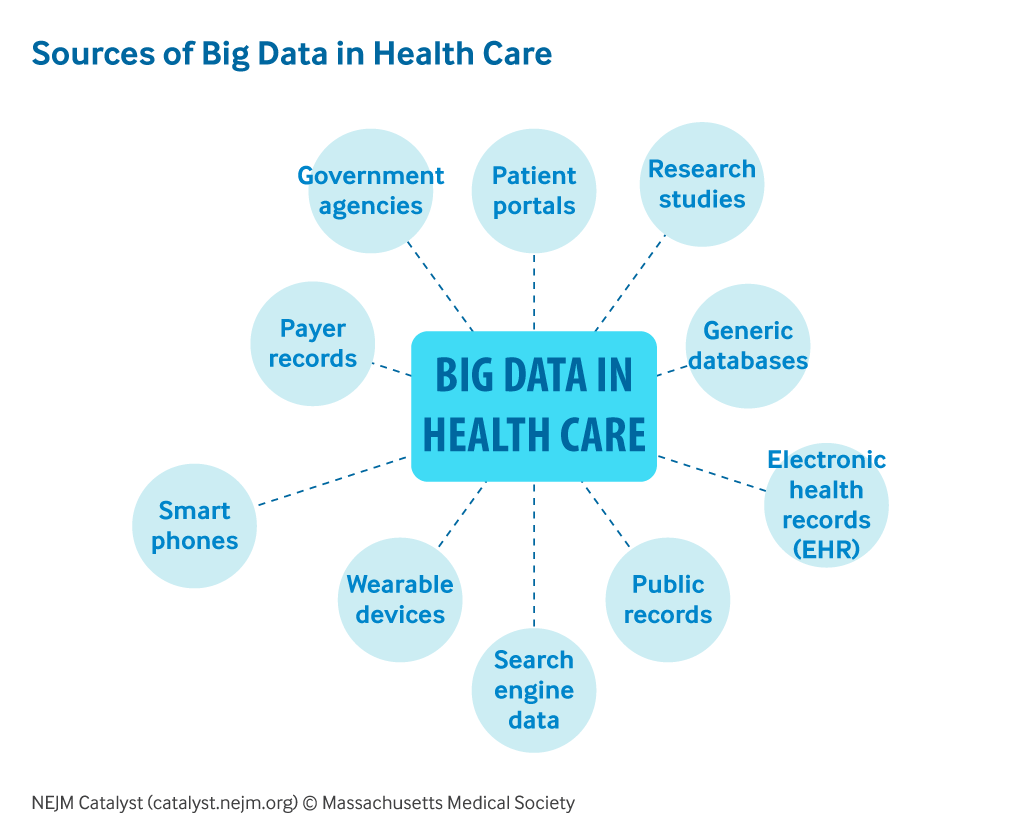
\includegraphics[width=0.75\linewidth,height=0.25\textheight]{images/big-data-healthcare} 

}

\caption{Big Data in Healthcare}\label{fig:sample-fig1}
\end{figure}

\hypertarget{introduction}{%
\section{Introduction}\label{introduction}}

~~~~~It has been estimated that roughly 80\% of health care data is
unstructured data, which can come in the form of videos, sensor data,
images, or text. Although hospitals and researchers historically had a
hard time extracting insights from this type of data, with the recent
advances that have been made in data science and handling big data, this
has created new application areas within the health care industry in
sectors such as genomics, predicting patient health, and medical imagery
(See Figure 1 \citep{NEJM}). Medical imaging research in particular has
made significant progress recently with scientists being able to use
different machine learning algorithms to detect different types of
lesions and cancers from CT, MRI, and other types of scans. In
particular the advancements of convolutional neural networks have
enormous potential for different image detection problems. In particular
this type of network could be used to assist doctors and clinicians as
to whether or not someone has pneumonia by looking at their CT Scans,
which would in turn help reduce the amount of hours and amount of
expertise required to understand these scans.

When working with medical imagery data sets one of the first problems
someone may run into is how to process and handle these large data sets.
When trying to perform analysis on small and medium sized data sets
within R, one rarely runs into complications that would be attributed to
how R is loading and dealing with the data itself. While most of the
time one can load data into the R Studio environment without issues and
without having to worry about whether the entirety of our data can even
be loaded in, one may begin to run into complications the larger the
data set becomes. If one ends up crossing into the threshold where R can
no longer store all the data in an effective way, there are multiple
potential solutions in the forms of choosing random subsets of the data,
buying a computer with larger memory, or use parallelization and using
multiple clusters to perform the analysis. It is this solution of
choosing random subsets of data, using the Keras and Tensorflow R
packages, that will allow me to work with and convert large image files
into a form that models can be trained on them.

By working with Keras and Tensorflow, this will allow me to utilize a
large medical imagery data set that consists of CT scans of patients
with and without pneumonia. This data set will then be used to train and
create convolutional neural networks that will try to identify whether
or not someone has pneumonia from the images.

This project will allow me to answer the questions of how does one
handle and process images so that analysis can be performed on them? How
does one create and train a convolutional neural network? And finally,
how effective are convolutional neural networks at identifying pneumonia
within CT scans?

\hypertarget{image-transformation-and-tensorflow}{%
\section{Image Transformation and
Tensorflow}\label{image-transformation-and-tensorflow}}

~~~~~Once the images are in a place where they could be loaded into R,
one needs to standardize the images into a format where R can actually
perform analysis on them. For images, this means making it so they all
have the same underlying features. This means performing different image
transformations such as cropping, brightness, contrasting, changing the
color scale, or resizing an image. This sort of data augmentation, when
performed on all the images in the data set can help create a more
consistent and standard form between all the images. For the images in
my medical imagery data set,this consisted of resizing the images on a
pixel by pixel basis so they were all the same size, and then converted
them to a grayscale color. When looking at Figure 2, we can see an
example of two different types of scans, one of a patient with pnuemonia
and one of a normal patient, but both have been converted to the same
size with the same contrast, brightness, and color scale.

\begin{figure}
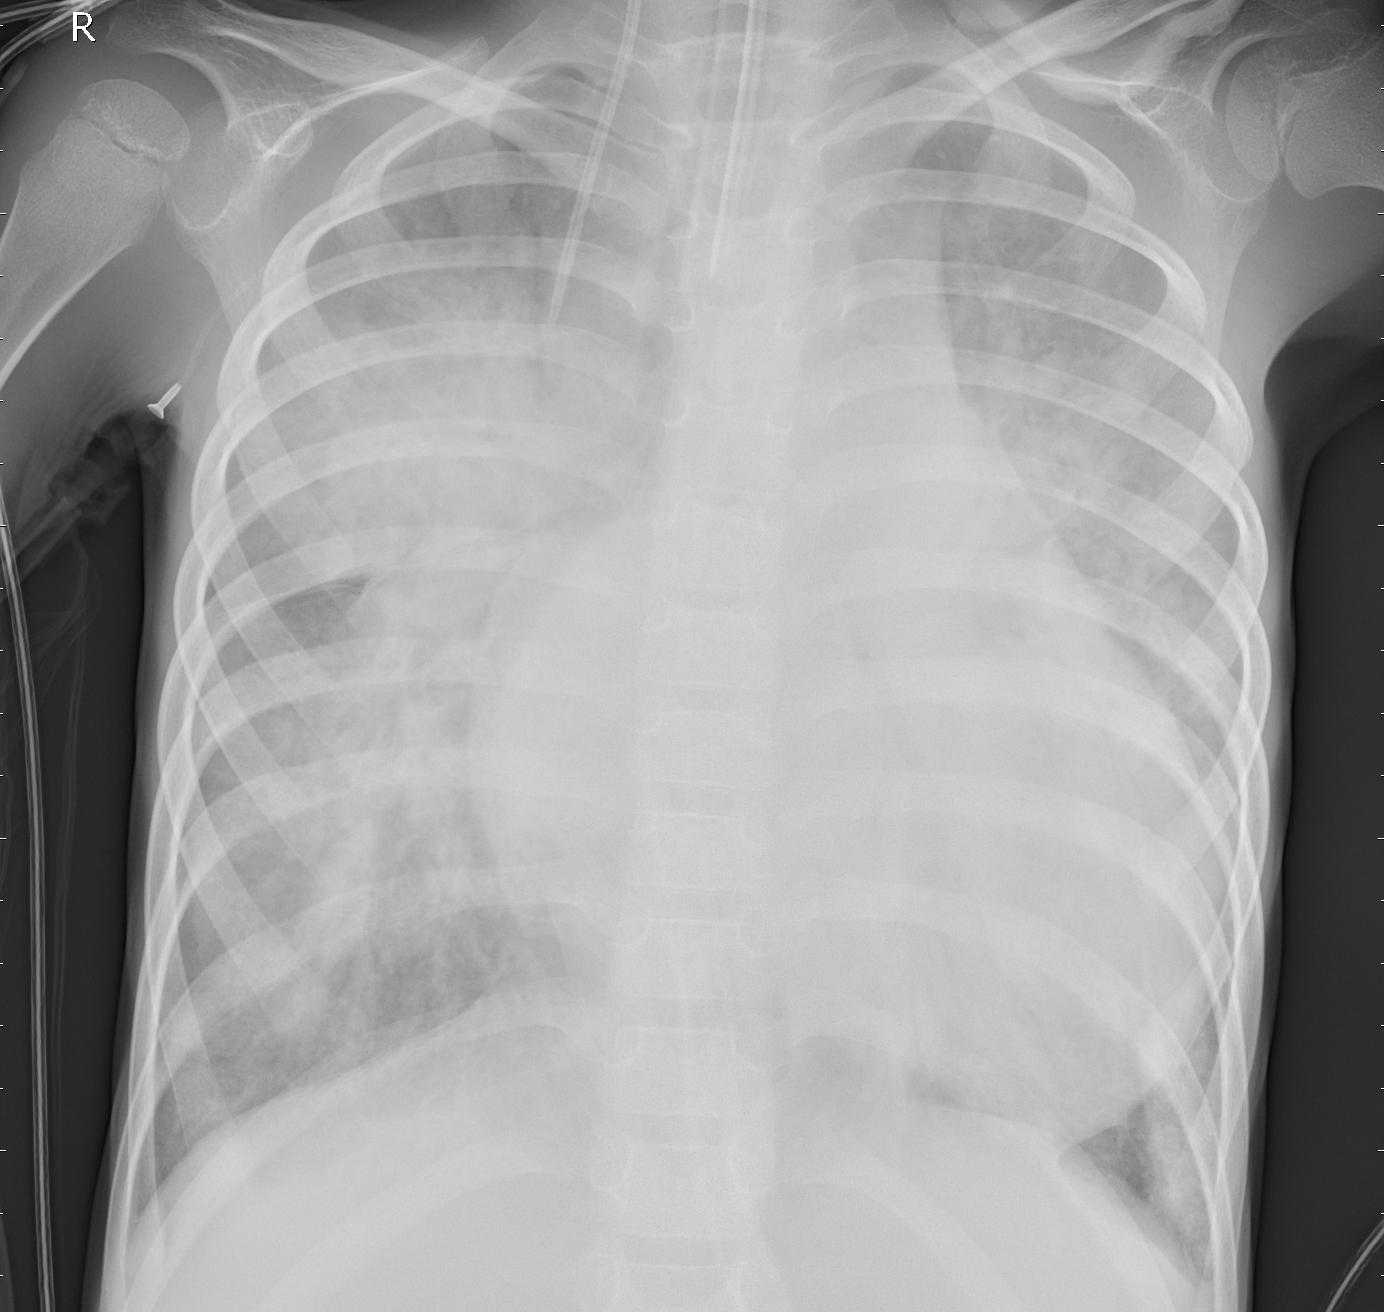
\includegraphics[width=0.49\linewidth,height=0.25\textheight]{images/pneumonia} 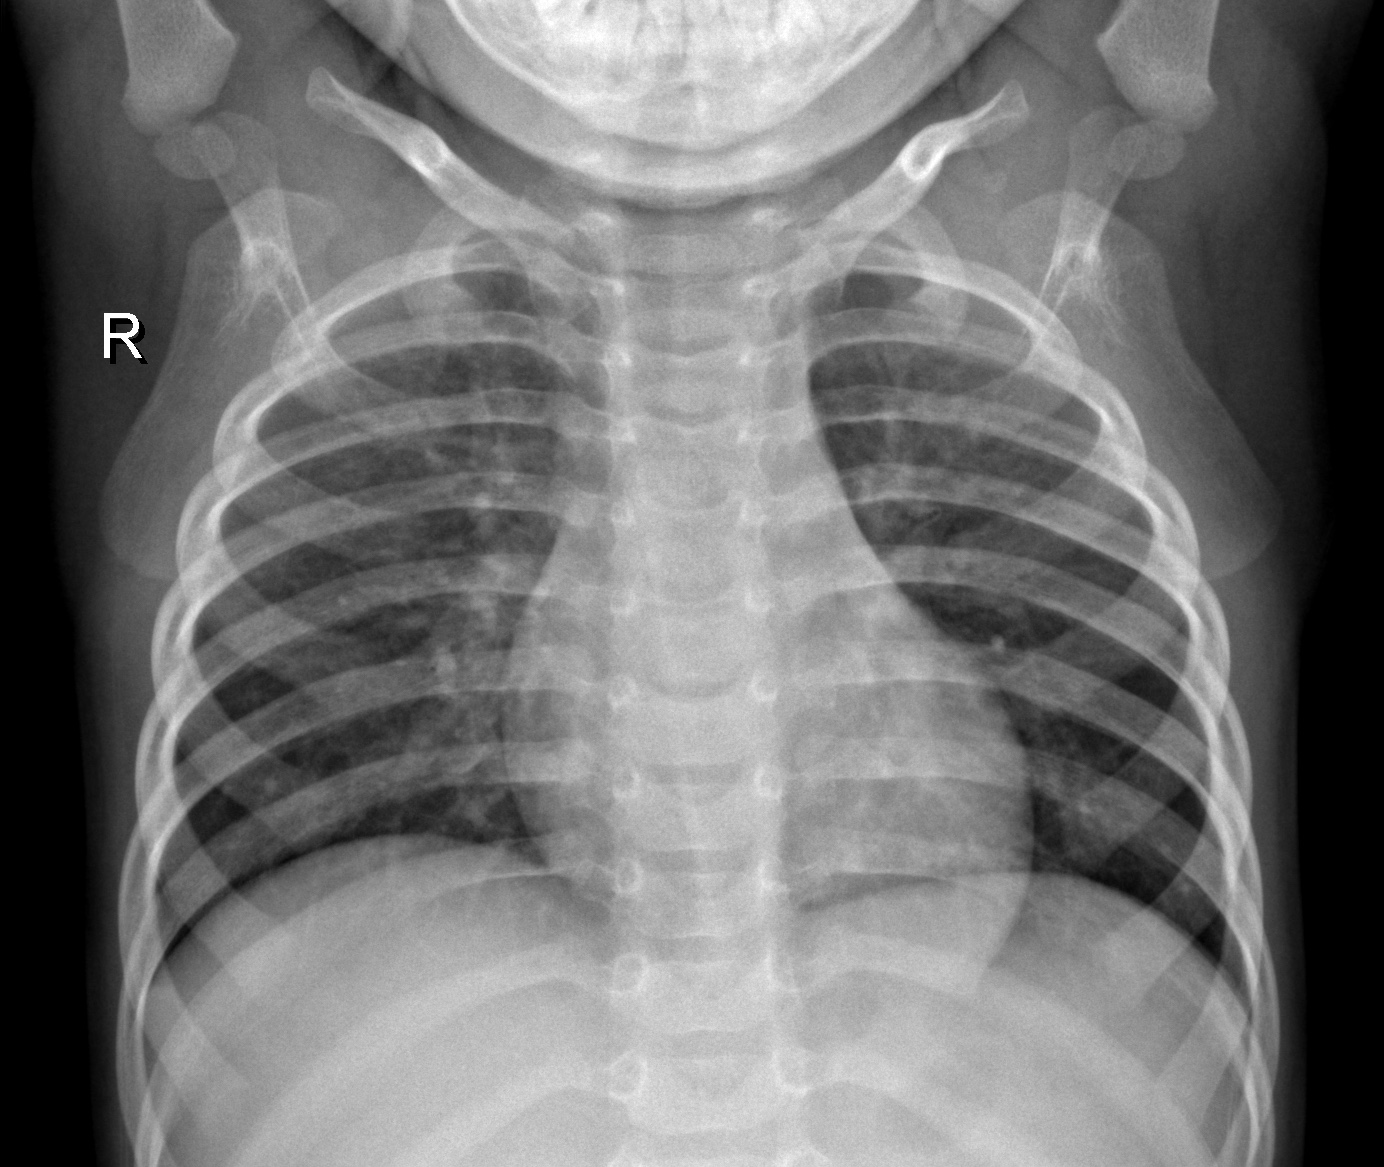
\includegraphics[width=0.49\linewidth,height=0.25\textheight]{images/normal} \caption{Patient CT Scans. At left, patient with pneumonia. At right, a patient without pnuemonia}\label{fig:sample-fig2}
\end{figure}

After getting all the images into the same structure, I needed to
convert them to a form where I could actually perform analysis on the
images. In order to do this I relied on the \emph{tensorflow} R package
\citep{Tensorflow2}. Tensorflow is a ``scalable and multiplatform
programming interface for implementing and running machine learning
algorithms'' \citep{PML}. This package is built around the idea of a
``computation graph composed as a set of nodes where each node
represents an operation''. A tensor is created as a symbolic handle to
refer to the input and output of these operations'' \citep{PML}. A
tensor is best understood as either a scalar, vector, or matrices where
all values within the tensor hold an identical data type. These tensors
are created from the values in the data and then are used to build and
create the complex models one wants to work with.

For the images in my data set, by using Tensorflow I was able to convert
the images into a set of tensors that represented the pixels of the
images themselves. Since the images had been resized to a 64x64 pixel
picture in grayscale coloring, this became a 64x64x1 tensor for each
image. These tensors were then combined with their appropriate label for
the type of image they were, either Normal or Pneumonia, creating a
nicely formatted data set where we could then start to create models to
best classify the data.

\hypertarget{keras-and-convolutional-neural-networks}{%
\section{Keras and Convolutional Neural
Networks}\label{keras-and-convolutional-neural-networks}}

~~~~~As we could see from the prior pictures of someone who had
pneumonia versus someone who did not have pneumonia, it can be very hard
to discern whether or not someone has pneumonia for a person without the
technical training and expertise to identify pictures of pneumonia from
looking at the CT scans. This ultimately requires doctors and those with
the expertise to spend more time looking at the scans, rather than
spending their already limited time directly helping patients. One way
to help doctors to get back to directly helping patients is by utilizing
machine learning to identify and detect different diseases or ailments
within CT scans. By training and creating models that are able to
discern between a normal or healthy scan versus someone who has a lesion
or has pneumonia, we can begin to use artificial intelligence to
alleviate some of the extraneous work that doctors are required to do.

\hypertarget{keras}{%
\subsection{Keras}\label{keras}}

~~~~~For this project, I was specifically focused on creating a model
that would would be able to discern between someone who has pneumonia
versus someone who does not have pneumonia. In order to do this I
utilized the \emph{keras} package in order to build a convolutional
neural network to be able to distinguish between the two different
diagnosis \citep{Keras2}. Keras is a ``high-level neural network API
that is built to run off other libraries such as Tensorflow to provide a
user-friendly interface to building complex models'' \citep{PML}. Keras,
when working with Tensorflow, helps to provide the framework to begin
building complex neural network models. This package will allow me to be
able to not only train and build the model, but also be able to predict
whether or not someone has pneumonia from looking at a specific image.

\hypertarget{neural-networks}{%
\subsection{Neural Networks}\label{neural-networks}}

\begin{figure}

{\centering 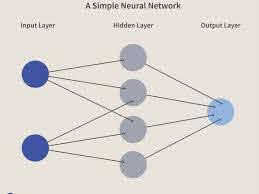
\includegraphics[width=0.75\linewidth,height=0.25\textheight]{images/neural_net} 

}

\caption{Structure of a Neural Network}\label{fig:sample-fig3}
\end{figure}

~~~~~By utilizing the Keras package, I was able to leverage a deep
learning technique called a neural network that has been proven to work
well on complicated machine learning tasks. Neural networks are
extremely popular today due to recent advances in both the algorithms
used to build the models as well as the computer architecture which
allows for much faster processing times of these complex models.

By looking at Figure 3, we can see an example of what the underlying
structure of a neural network looks like (See Figure 3
\citep{Investopedia}). The neural network shown in this example consists
of one input layer, one hidden layer with 4 hidden units, and then one
output layer. The input layer would be the exact data you are feeding
into the model, so for this picture this would mean there was two
examples being fed into network to train the model. Then we can see how
each of the input layers are connected to three of the gray nodes in the
hidden layer. Then finally there is one output layer that is connected
to all the nodes of the hidden layer. In general, neural networks can
contain differing number of hidden layers, hidden units, and input and
output units, which will all depend based on the data they have and the
problem one is trying to solve. Although these models can be extremely
hard to interpret and understand, they have been shown to be extremely
successful at a broad range of tasks from natural language processing to
self-driving cars.

\hypertarget{convolutional-neural-networks-cnn}{%
\subsection{Convolutional Neural Networks
(CNN)}\label{convolutional-neural-networks-cnn}}

\begin{figure}

{\centering 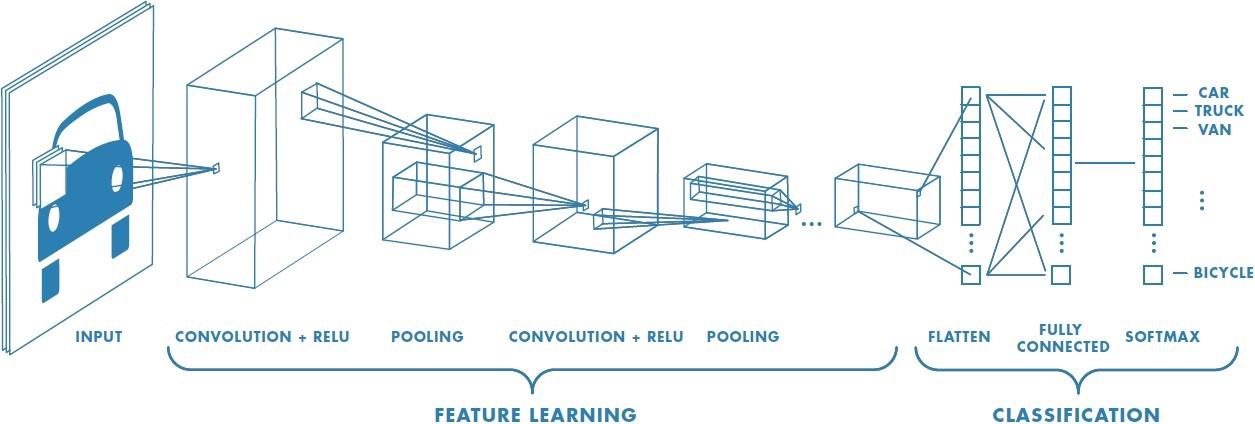
\includegraphics[width=0.75\linewidth,height=0.25\textheight]{images/cnn} 

}

\caption{Convolutional Neural Network Example}\label{fig:sample-fig4}
\end{figure}

~~~~~The specific form of neural network that I utilized for my project
was a Convolutional Neural Network. Convolutional Neural Networks (CNN)
at a high level are a form of deep learning that takes an image as an
input and eventually classifies it under a certain category. These types
of networks are used heavily to perform tasks such as facial
recognition, object detection, and image classification to just list a
few. CNN's are based heavily on how the visual cortext of the human
brain works when recognizing images, which is what allows it to perform
extremely well on image classification tasks.

CNN's work by ``combining the low level features in a layer-wise fashion
to form high-level features'' \citep{PML}. So rather than just looking
at each pixel of an image separately, this model works to combine pixels
into distinct features that can then be used to identify exact objects
within the images. In order for the model to actual identify distinct
features it relies on an idea called feature mapping that groups patches
of pixels together in the image and combines them into one feature in
the new feature map. This is based on the underlying assumption that in
the context of image data, ``nearby pixels are typically more relevant
to each other than pixels that are far away from each other''
\citep{PML}.

In order to actually perform this feature mapping though a CNN relies on
creating a series of different types of layers in the form of
convolution layers, subsampling layers, pooling layers, and dropout
layers. By looking at Figure 4, one can begin to understand how the
different layers connect to form a model \citep{CNN}.

\hypertarget{convolution-layers}{%
\subsubsection{Convolution layers}\label{convolution-layers}}

~~~~~Convolution layers is one of the first layers that begins
extracting features from the input images. This layer works by taking an
input matrix that represents the image, and a filter matrix, of
potentially a different size. These two matrices are multiplied together
to create a feature map that begins to identify the low level features
such as edges, blurriness, or sharpness of the image.

\hypertarget{subsampling-and-pooling-layers}{%
\subsubsection{Subsampling and Pooling
Layers}\label{subsampling-and-pooling-layers}}

~~~~~Another type of key layers are the subsampling and pooling layers.
Usually the feature map that is created from the previous convolution
layer is then fed into a subsampling or pooling layer. These layers work
by combining small subsections of the feature map in order to simplify
the feature map. The advantages of this include leading to higher
computational efficiency by decreasing the size of the features and the
number of parameters that are required to learn, as well as introducing
local invariance that helps to generate features that are more robust to
noise from the input images \citep{Mathworks}.

\hypertarget{dropout-layers}{%
\subsubsection{Dropout layers}\label{dropout-layers}}

~~~~~Dropout layers are then used to prevent over-fitting of the data
set. It can be very easy to create a CNN that gets over-trained but then
fails to perform well on the testing set of data. To prevent
over-fitting and make the model work well for a broader range of images
for general performance, dropout layers are introduced as a form of
regularization. Dropout is usually applied to units of hidden layers and
works by ``during the training phase of a neural network, a fraction of
the hidden units are randomly dropped at every iteration. This dropping
out of random units requires the remaining units to rescale to account
for the missing units which forces the network to learn a redundant
representation of the data'' \citep{PML}. This makes it so the model is
more generalizable and robust to changes in patterns in the data and
prevent over-fitting.

\hypertarget{challenges}{%
\subsubsection{Challenges}\label{challenges}}

~~~~~When working with CNN's, these different types of layers that the
network can be built off of can all be included multiple times and in
different orders. For example one could create a network of just a
convolution layer and a dropout layer or someone could create a model
that is convolution layer, pooling layer, convolution layer, and then
two dropout layers. There is no set rules around what order or how many
different layers your network can have. On top of having unlimited
variations of the type of layers within the network, there is also
unlimited parameters that one can choose in terms of the size of the
feature map, the number of units to pool together in the pooling layer,
or the number of units to dropout in the dropout layer to just list a
few examples. Due to having so many input parameters that can be changed
and altered when it comes to building the model, finding the best
possible input parameters and underlying structure of the model can
become computationally expensive very quickly.

~~~~~On top of CNN's being very computationally expensive to run, being
able to interpret the outputs and inputs of individual layers of the
network is its own separate issue. Often these types of models are
referred to as ``black box'' models because while a human can understand
the input and outputs of the models, it is often hard to decipher and
understand what exactly the model is doing inside the box. For example,
it is very tough to understand exactly how the model is able to
distinguish between someone who has pneumonia or not. While there has
been promising developments in this area such as Visualizing Activation
Layers and Occlusion Sensitivity, this still remains an area of the
field that a lot of future work can be done in \citep{Deep}. While CNN's
have been shown to do an incredible job at image classification tasks,
optimizing and understanding these types of models is an area that can
cause problems and issues.

\hypertarget{cnns-with-medical-images}{%
\subsection{CNN's with Medical Images}\label{cnns-with-medical-images}}

~~~~~For my project, I wanted to use Convolutional Neural Networks to
see how well this type of network could perform on the task of trying to
classify whether or not someone had pneumonia based just of a CT scan.
At this point I have already gotten my images into a form that allows
them to be passed as inputs to build a model, so the next step was for
me to begin training the model.

To begin training the model I started off by first splitting my data
into training, validation, and testing sets. The training set would be
used to train the model, the validation set would be used to tune the
parameters in the network, and then the test set would then be used to
assess the performance of the final model and see how generalizable the
results are when given separate input images.

After splitting up the data into their different sets I found that
overall the data set contained many more pictures of people than
pneumonia than people who did not have pneumonia. In fact, the training
data contains 74\% picture of people with pneumonia and 26\% being
normal images.

What this tells us is that if a random person were to guess that every
picture was a picture of pneumonia, that they would be correct 74\% of
the time. So when I build out my models, I will be looking for a model
that is able to achieve better than 74\% accuracy to say it is an
improvement over a baseline random guessing model.

\hypertarget{model-1}{%
\subsection{Model 1}\label{model-1}}

~~~~~Now that I had an understanding of what my training set looked
like, I wanted to try building my first convolutional neural network.
For my first model I decided to build a model that had one convolution
layer, one pooling layer, one flattening layer, a dropout layer that
removed half of the available units available in the previous layer
during each new training iteration, and then finally one dense layer.
The flattening layer works to replace all dimensions of the previous
tensors down to one dimension, which is the dimension size we want our
output layer to be. The dropout layer is used to make the model more
generalizable and requires the model to fit the units with only half the
units of the previous layer available during any iteration. The final
dense layer is used to create a layer of units, in this case one unit,
where every unit in this new layer is connected to every unit in the
previous layer, making it densely connected. By looking at Figure 5, one
can see what this model looks likes, and how there are 13,121 trainable
parameters. These are all the weights between the different layers that
the model will try to optimize during each training run.

\begin{figure}

{\centering 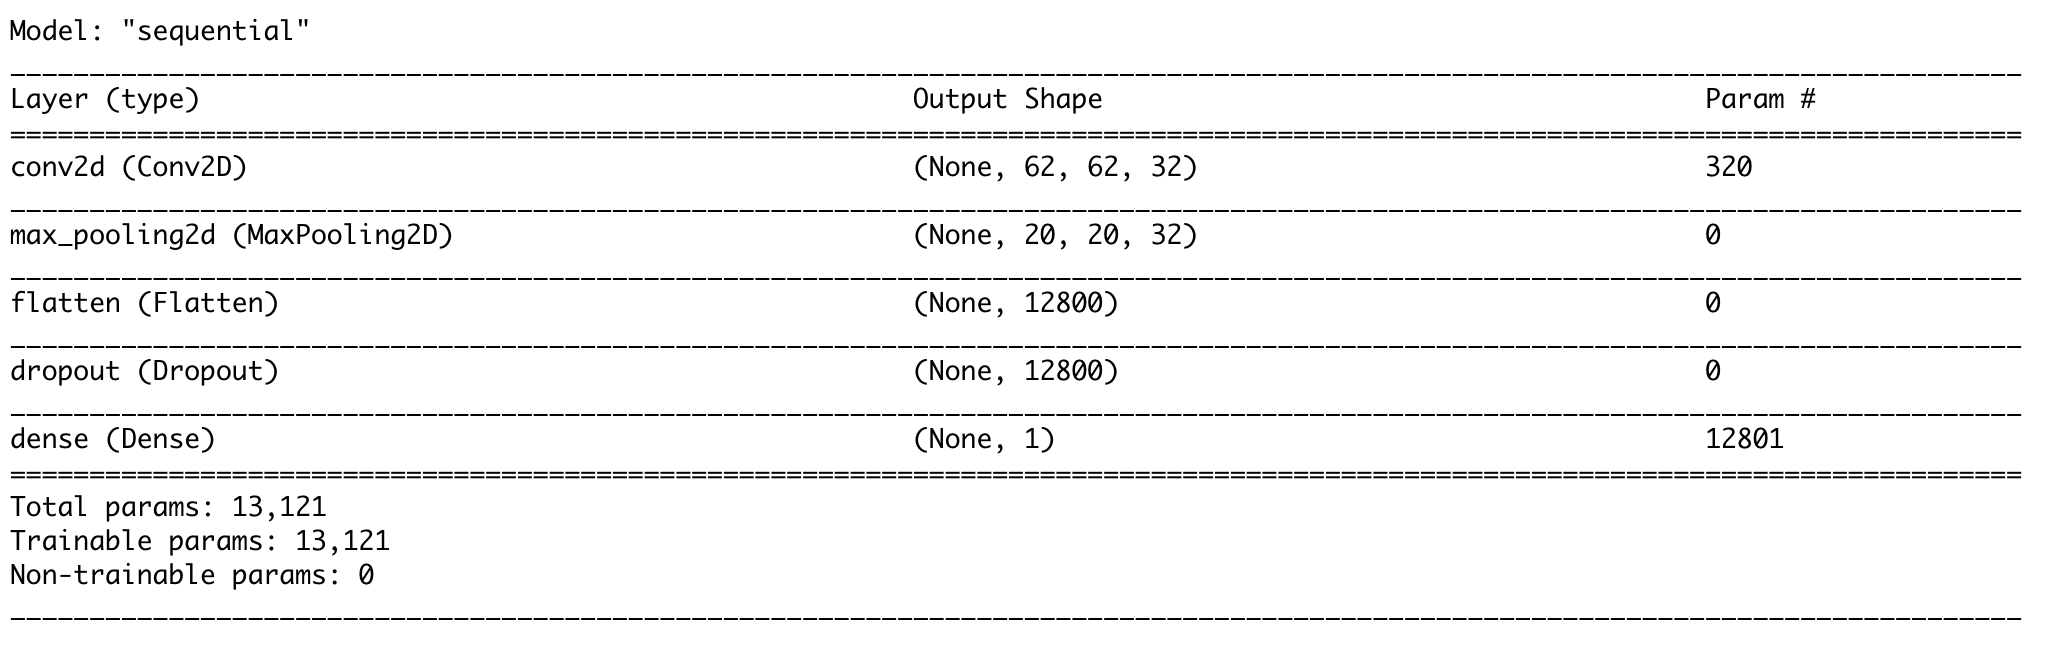
\includegraphics[width=0.75\linewidth,height=0.25\textheight]{images/model1} 

}

\caption{Summary of Model 1}\label{fig:sample-fig5}
\end{figure}

After training this model we can see from looking at Figure 6 that
although it starts at around being 75\% accurate on both the training
and validation sets, that even after 5 epochs that the model does not do
any better at being able to discern between whether or not an image is
normal or pneumonia than just random guessing. This suggests that either
the model does not have enough layers to it and is not able to extract
distinguishable features from the images or that there were not enough
epochs to train the model. It is also worth noting that this model took
2 and a half minutes to complete its training, with roughly 30 seconds
per epoch. This long run time is due to the large number of trainable
parameters in the model.

\begin{figure}

{\centering 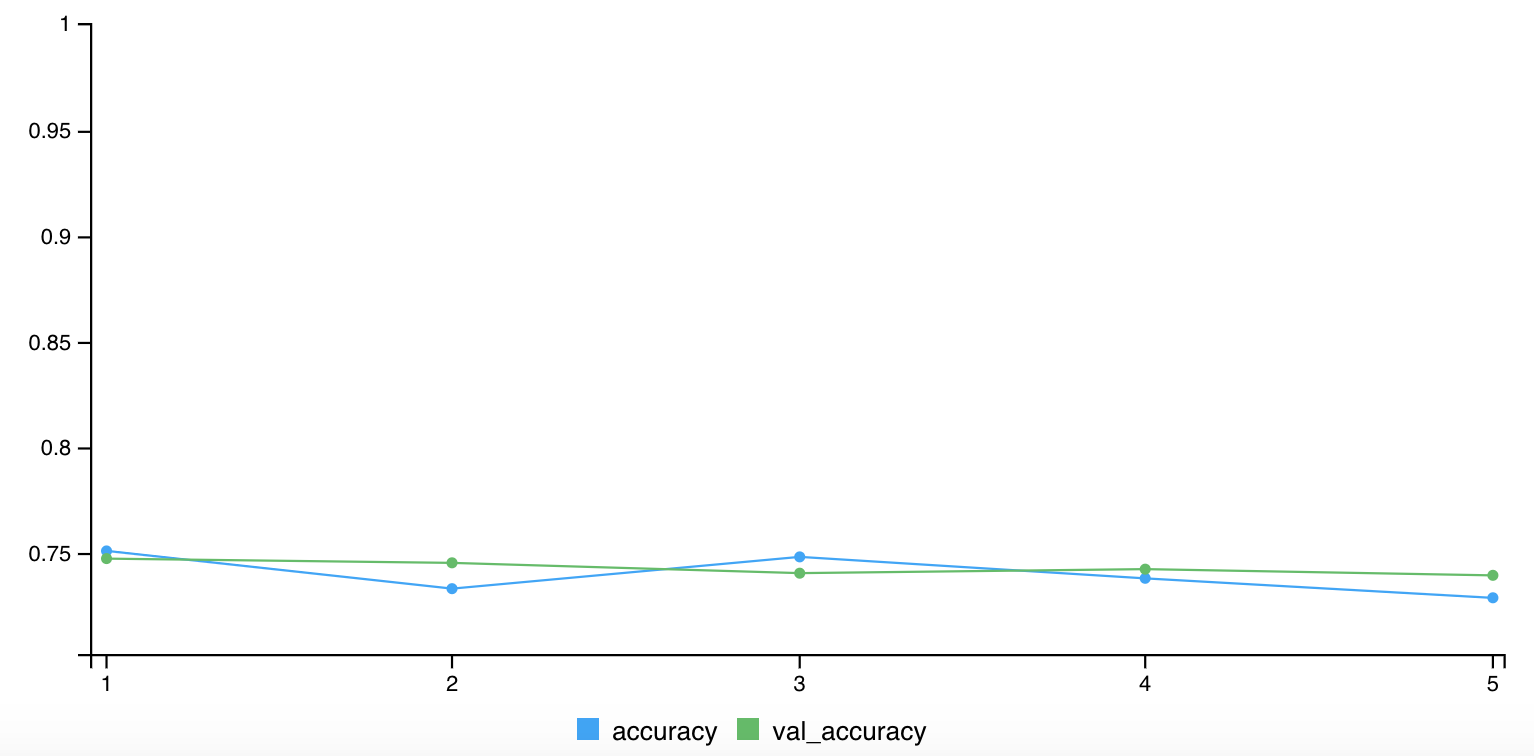
\includegraphics[width=0.75\linewidth,height=0.25\textheight]{images/model1out} 

}

\caption{Model 1 Accuracy per Epoch}\label{fig:sample-fig6}
\end{figure}

\hypertarget{model-2}{%
\subsection{Model 2}\label{model-2}}

~~~~~Since model 1 did not do any better than one would do than just
randomly guessing, I decided to try to improve upon the first model by
adding a second convolution layer after the first pooling layer, as well
as a second dense layer at the end of the model. I also decided to
increase the number of epochs from 5 to 10 to see if allowing the model
a longer period of time to train itself would help improve the accuracy
of the model at all. My hopes were that adding these new layers would
help the model discover features in the images that it wasnt able to
detect with the first model and adding more epochs would give the model
more time to find these features. Figure 7 shows how the new model is
constructed. We can see that by adding these two new layers to the model
that there are now 34,659 parameters that the model is going to try to
maximize during its training process.

\begin{figure}

{\centering 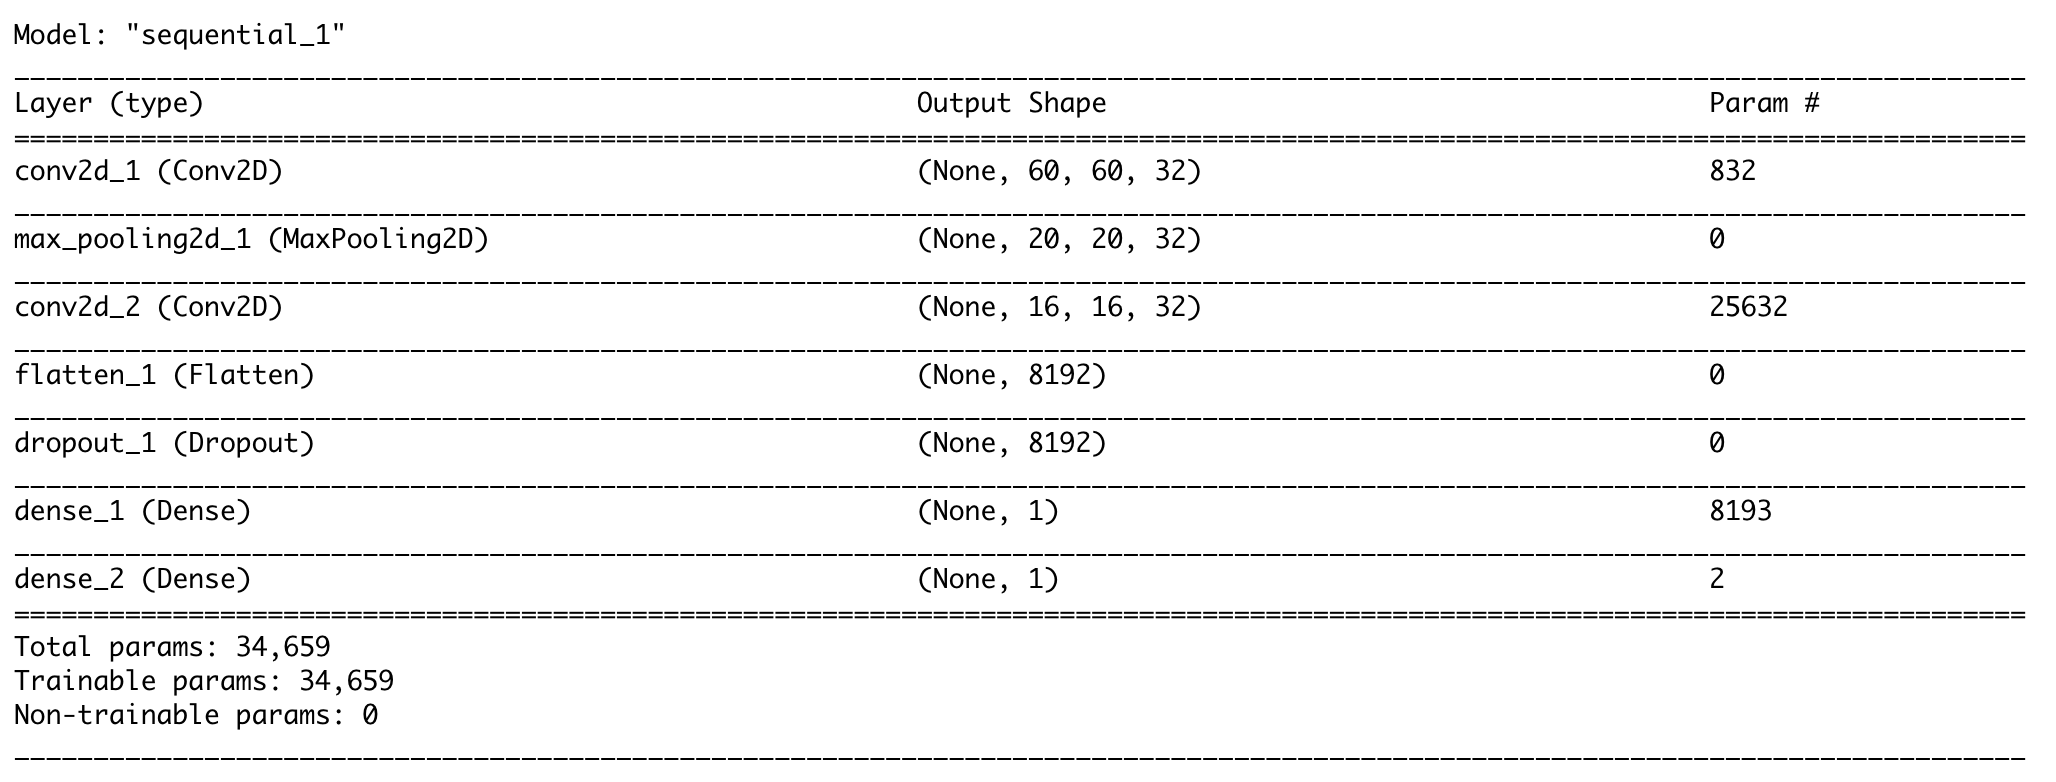
\includegraphics[width=0.75\linewidth,height=0.25\textheight]{images/model2} 

}

\caption{Summary of Model 2}\label{fig:sample-fig7}
\end{figure}

\begin{figure}

{\centering 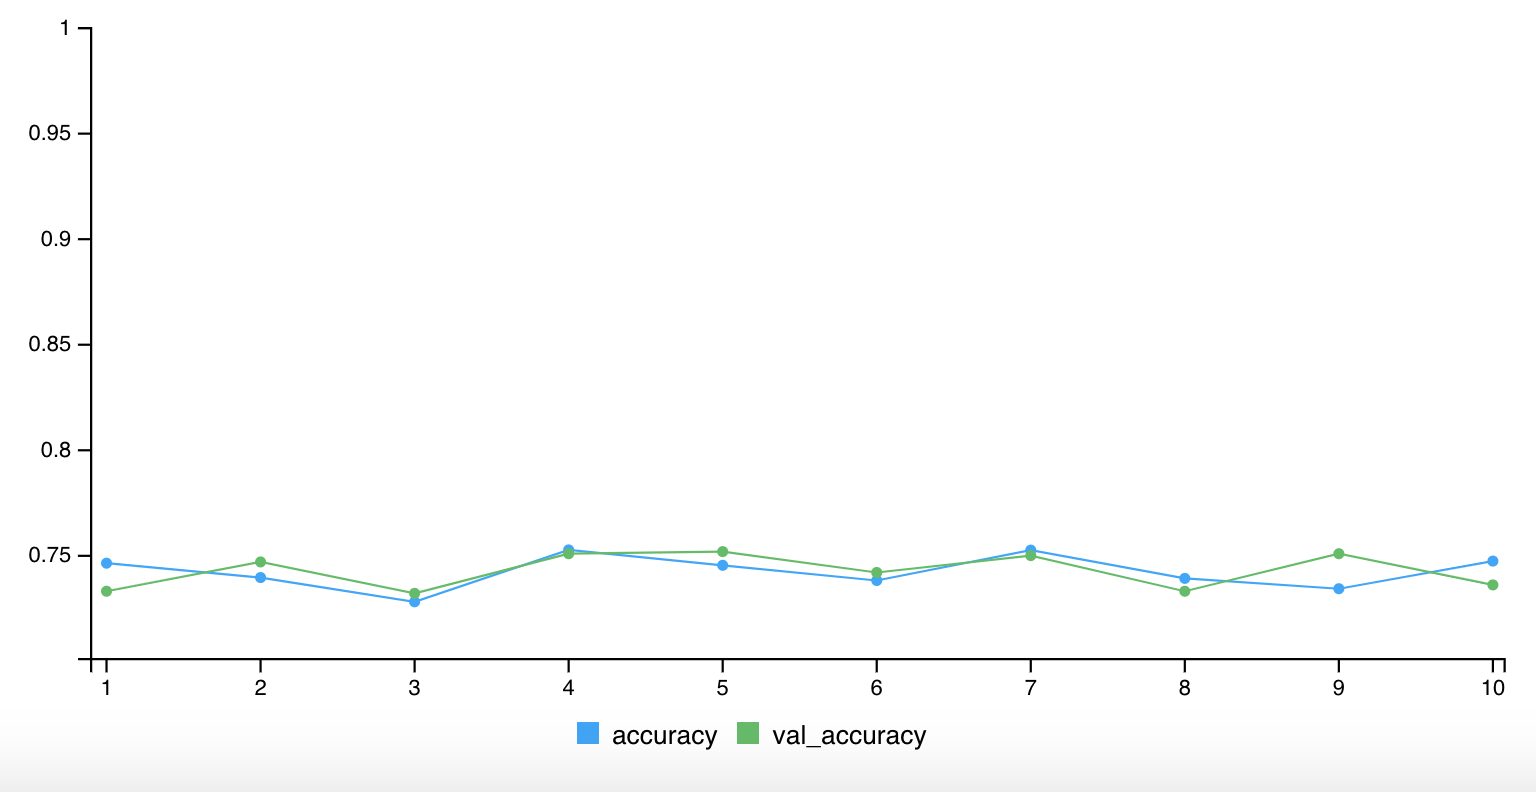
\includegraphics[width=0.75\linewidth,height=0.25\textheight]{images/model2out} 

}

\caption{Model 2 Accuracy per Epoch}\label{fig:sample-fig8}
\end{figure}

Even after adding a second convolution layer and a second dense layer at
the end, we can see that this model again does not do any better than
the previous model by looking at Figure 8. One can see that the accuracy
stays right around 75\% for both the training and validation sets, and
that even after increasing the complexity of the model slightly and
increasing the number of epochs that the model is still not any better
than guessing Pneumonia every time. This model also took roughly 5
minutes to run with every epoch taking 30 seconds to run.

\hypertarget{model-3}{%
\subsection{Model 3}\label{model-3}}

~~~~~Since my second model still did not do much better than someone
randomly guessing, for my third model I decided to increase the
complexity of the model substantially. Since the previous models did not
appear to be able to detect any distinguishable features from the
images, by increasing the number of layers in the model I believe it
should help the model finally be able to detect the underlying features.
For this model I decided to have 4 pairs of convolution, pooling, and
dropout layers, followed by a flattening layer and then two dense
layers. As we can see from Figure 9, this model now has 98,017 trainable
parameters that the model will try to optimize.

As we can see from this output, the model is finally able to discern
between images that contain pneumonia and normal images. As we can, over
the course of 10 epochs the model is able to increase it accuracy from
under 75\% to close to 90\% by the 10th epoch. From the graph we can
also see that the validation accuracy score is always slightly under the
training accuracy score, which suggests that the model might be slightly
over-fitting the data, but because I already included 4 dropout layer in
the model and the scores are still relatively close, this is not
something to worry about too much. This model also took close to 5
minutes to run even though the number of trainable parameters increased
substantially.\\

\begin{figure}

{\centering 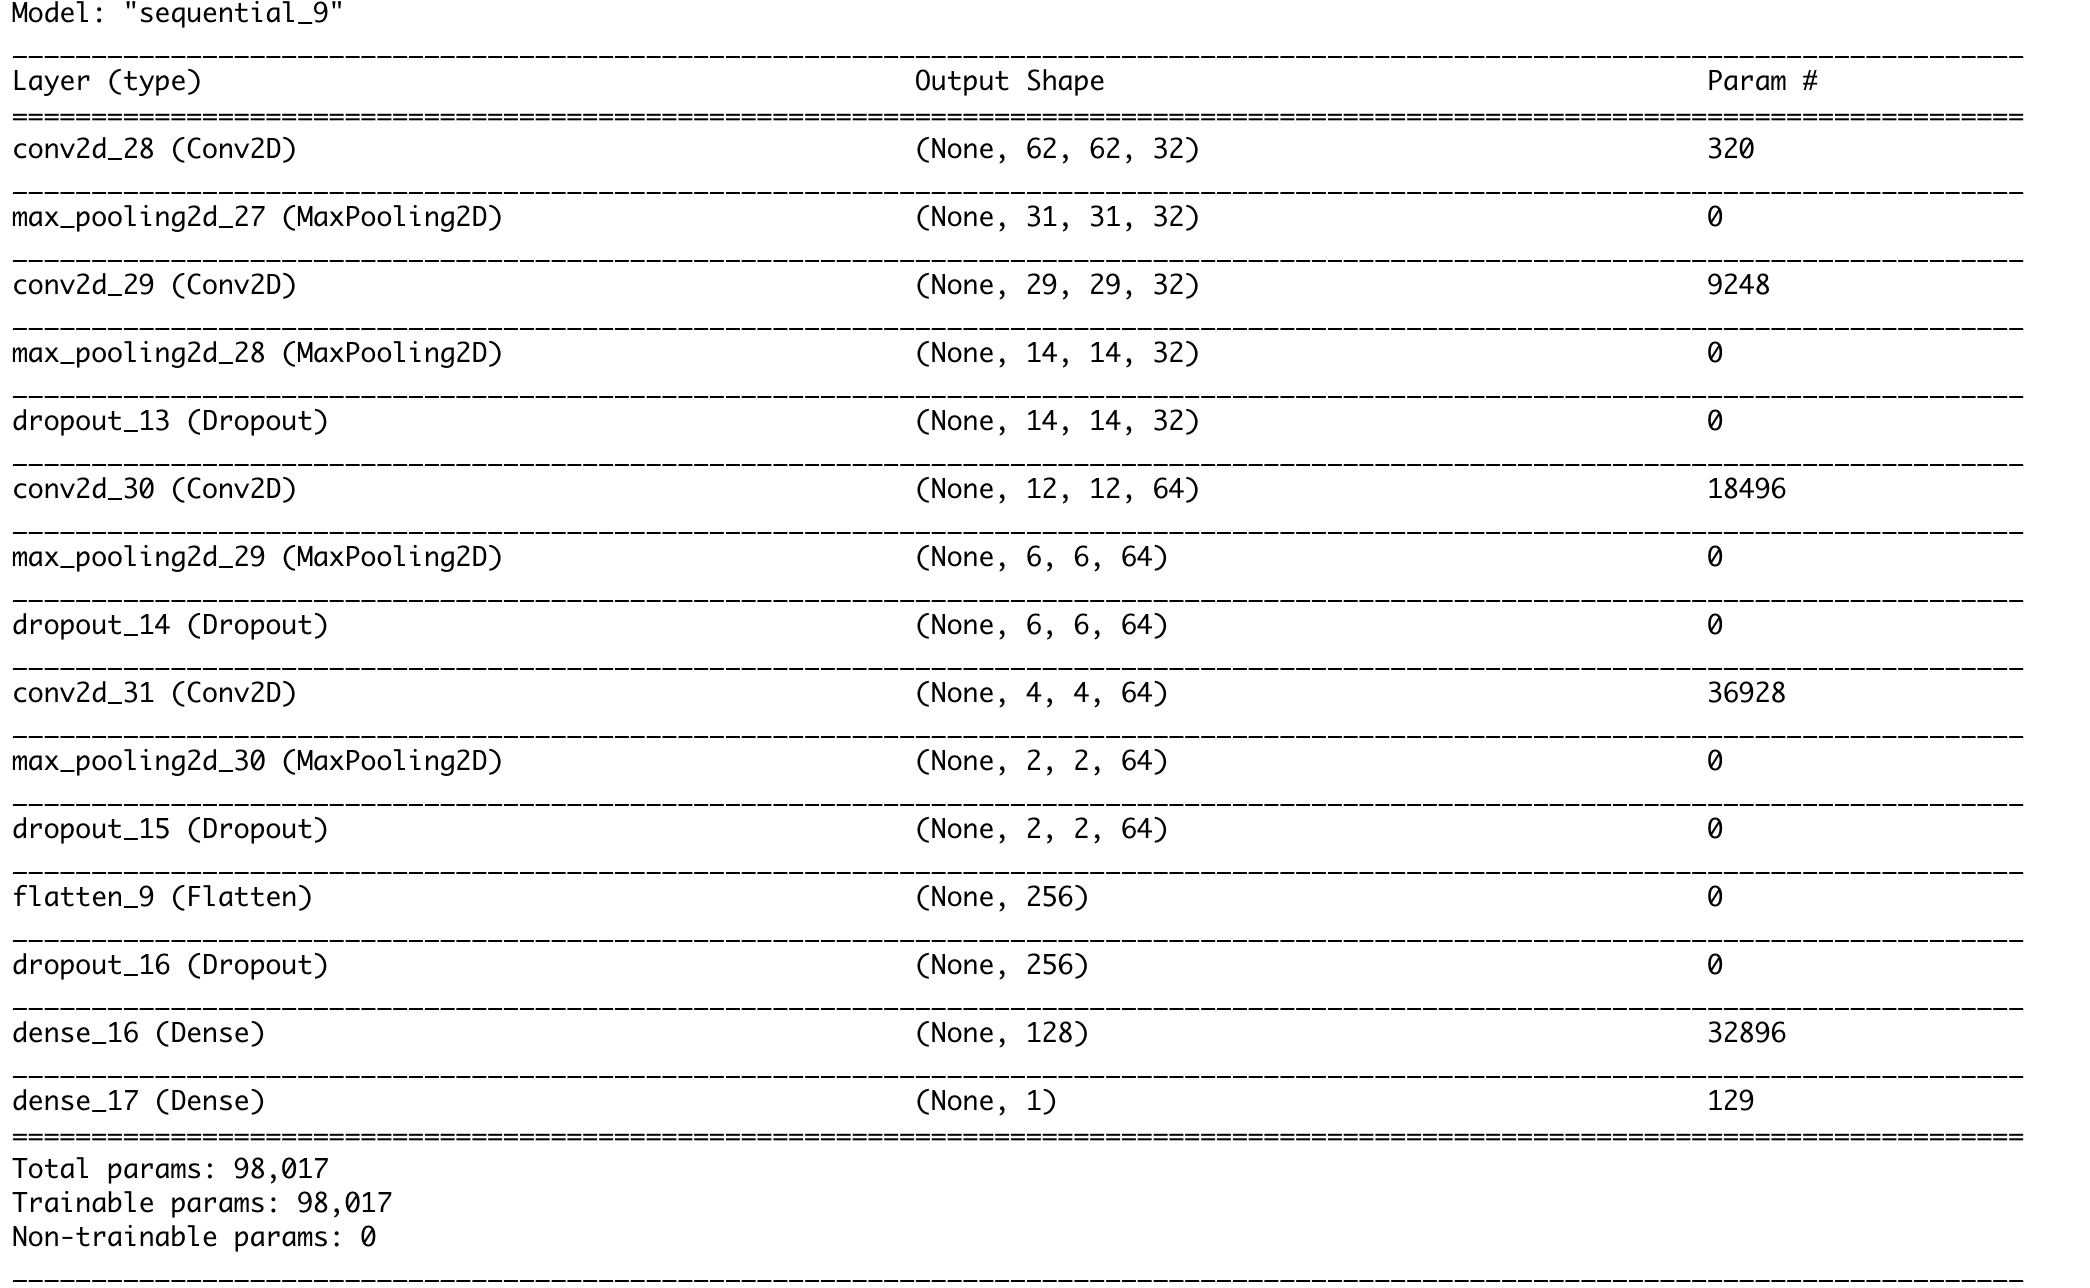
\includegraphics[width=0.75\linewidth,height=0.25\textheight]{images/model3} 

}

\caption{Model 3 Summary}\label{fig:sample-fig9}
\end{figure}

\begin{figure}

{\centering 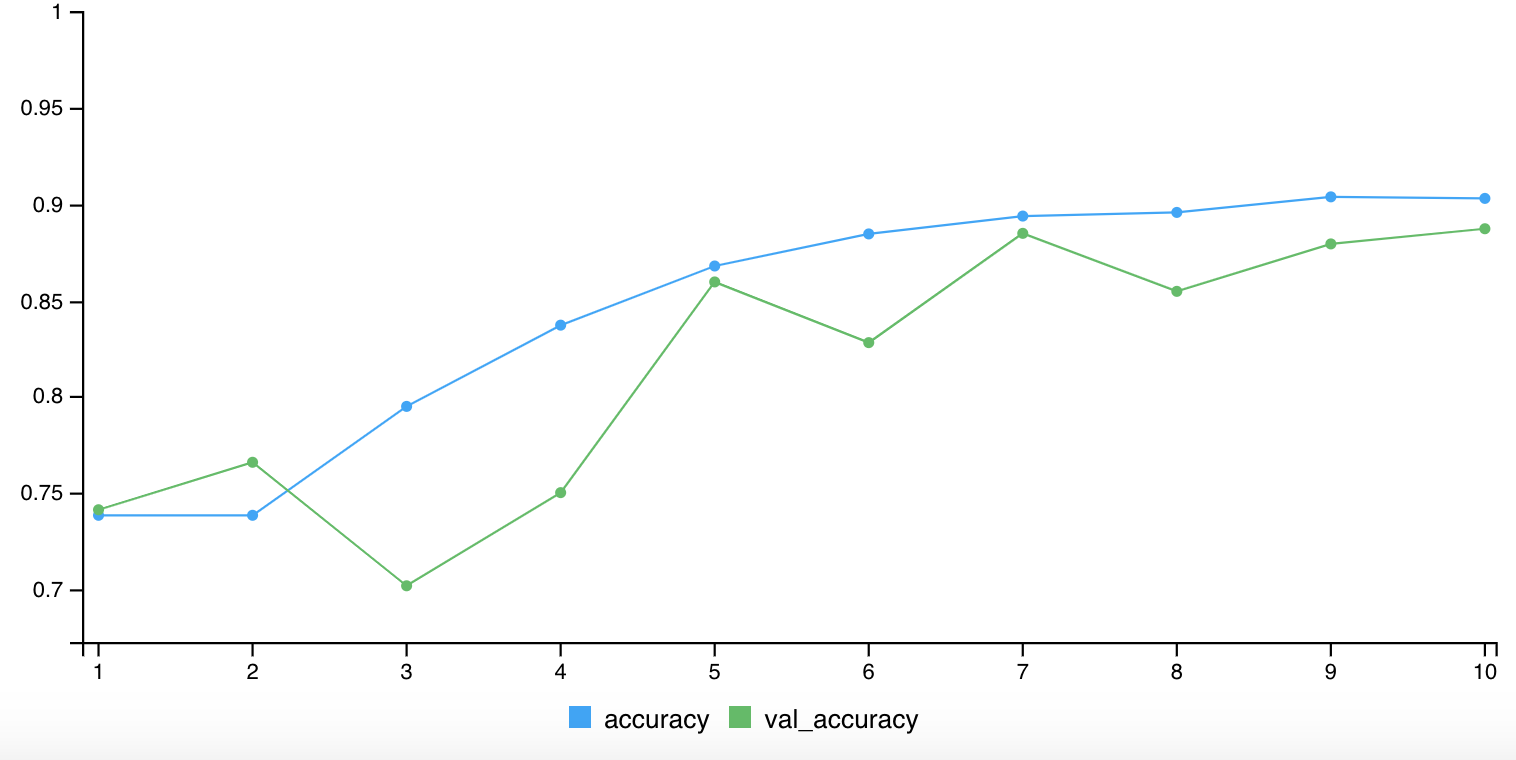
\includegraphics[width=0.75\linewidth,height=0.25\textheight]{images/model3out} 

}

\caption{Model 3 Accuracy}\label{fig:sample-fig10}
\end{figure}

\hypertarget{results}{%
\subsection{Results}\label{results}}

~~~~~~After creating each of these three different models, we can see by
looking at the chart below, that Model 3 is able to obtain the highest
accuracy scores on both the training and validation sets. Therefore I
will use this model on the testing set. ~

\begin{tabular}{l|r|r}
\hline
Model & Training Accuracy & Validation Accuracy\\
\hline
Model 1 & 0.75 & 0.75\\
\hline
Model 2 & 0.75 & 0.75\\
\hline
Model 3 & 0.90 & 0.88\\
\hline
\end{tabular}

~~~~~After running model 3 on the testing set, the model was able to
achieve an accuracy score of 84.62\% and a loss score of 0.381 . The
testing set contained 234 normal images and 390 pneumonia images so if
one were to guess pneumonia every time they would be correct 62.5\% of
the time. While this model could potentially still be improved upon,
being able to train a model that achieves an accuracy of 85\% on a task
as challenging as being able to identify whether or not someone has
pneumonia is a very promising result. ~

\begin{tabular}{l|r|r}
\hline
Model & Accuracy & Loss \\
\hline
Model 3 & 0.846 & 0.381\\
\hline
\end{tabular}

While ideally I would like to understand how the model is making its
decisions, and understand exactly how each of the different layer is
affecting the output of the model, currently this task is extremely
challenging and is a major downside of using this type of model. As
briefly mention earlier, one of the biggest challenges with using this
type of model is being able to interpret the model itself and is why its
commonly referred to as a blackbox model. Being able to explain these
types of models is a huge area of research, and trying to go under the
hood and unpack the model could be its own separate project. For now
this means that I have to settle for looking at what types of scans the
models does a good job classifying, to see how it could be improved.

\begin{figure}

{\centering 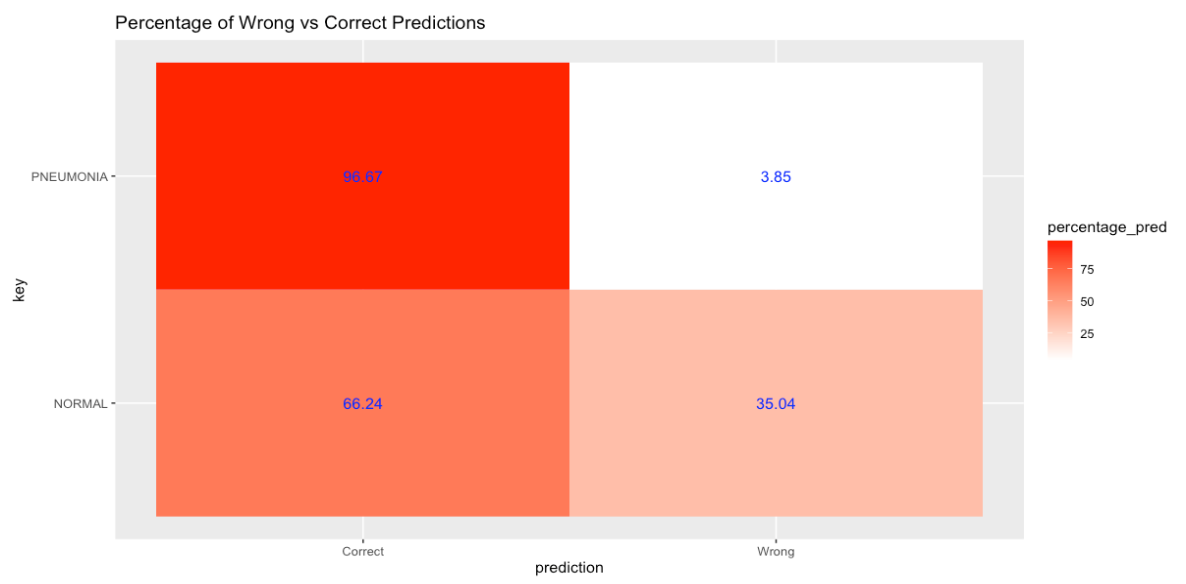
\includegraphics[width=0.75\linewidth,height=0.25\textheight]{images/heatmap} 

}

\caption{Confusion Matrix of Testing Set Results}\label{fig:sample-fig11}
\end{figure}

When looking at Figure 11, we can break down the accuracy score further
and look into how the model did at identifying the two different classes
one can begin to look into areas where the model does very well and
where the model struggles. By looking at the confusion matrix in Figure
11, we can see that the model does an extremely good job of identifying
when the image is of someone who has pneumonia, being able to predict is
correctly 96.7\% of the time. We can also see that the model is only
able to correctly predict whether someone is normal at a 66.2\% of the
time. What this output tells us is that the model is more likely to
identify a patient as having pneumonia when they have do not have it,
rather than the opposite scenario of telling a patient they do not have
pneumonia when they in fact have it which is probably the more dangerous
scenario. When thinking about why the model does such a better job at
identifying patients who have pneumonia, it comes back to the type of
data we used to train the model. Since the training and validation data
contained 3x as many pictures of pneumonia, it makes sense that the
model does a much better job of being able to recognize when someone has
pneumonia. So while being able to achieve 85\% accuracy with a
convolutional neural network is very promising, these results show that
there is future work that can be done that would be able to improve the
model's accuracy even more.

\hypertarget{conclusion-and-future-work}{%
\section{Conclusion and Future Work}\label{conclusion-and-future-work}}

~~~~~When reflecting back and thinking about ways that this worked could
be built on in the future, the first thing that comes to mind is
learning how to use different image augmentation techniques to build off
the underlying images. Having a training set that contained a much
higher percentage of patients with pneumonia than patients without
pneumonia drastically affected the final model that was created. As one
could see from the final confusion matrix, the model did an incredible
job correctly predicting when a patient had pneumonia but did poorly
when predicting if a patient was normal. This is largely due to the
training set that it was fed and is the first area that could be used to
improve the model.

The second way this project could be improved upon in the future would
have been to work entirely within the Google Cloud Environment. Since
Google Cloud now offers an R Studio that runs directly within their
cloud environment, this means that I could have taken advantage of both
Google Cloud Storage, to store the data, and also the Google Cloud AI
Platform, to optimize the model.

The Google Cloud AI Platform would have first helped by speeding up the
run time of the models I created. As I mentioned in the report, running
and training these models took upwards of 5 minutes each and this didn't
include any optimization techniques. Using the AI platform would have
allowed me to speed up the training time and also try out different
optimization methods that would have helped improve the accuracy of my
model even further. So while overall this project was very successful in
what I set out to learn, there are certainly still areas that could be
improved upon in the future.

\hypertarget{appendix}{%
\section{Appendix}\label{appendix}}

\hypertarget{image-transformation-and-tensorflow-1}{%
\subsection{Image Transformation and
Tensorflow}\label{image-transformation-and-tensorflow-1}}

\begin{Shaded}
\begin{Highlighting}[]
\NormalTok{chest_list <-}\StringTok{ }\KeywordTok{c}\NormalTok{(}\StringTok{"NORMAL"}\NormalTok{,}\StringTok{"PNEUMONIA"}\NormalTok{)}
\NormalTok{output_n<-}\KeywordTok{length}\NormalTok{(chest_list)}

\NormalTok{img_width <-}\StringTok{ }\DecValTok{64}
\NormalTok{img_height <-}\StringTok{ }\DecValTok{64}
\NormalTok{target_size <-}\StringTok{ }\KeywordTok{c}\NormalTok{(img_width, img_height)}

\CommentTok{#this is for grayscale images}
\NormalTok{channels <-}\StringTok{ }\DecValTok{1}

\NormalTok{batch_size<-}\DecValTok{32}

\CommentTok{# path to image folders}
\NormalTok{train_image_files_path <-}\StringTok{ }\KeywordTok{file.path}\NormalTok{(}\StringTok{"setup/images/chest_xray/train"}\NormalTok{)}
\end{Highlighting}
\end{Shaded}

\begin{Shaded}
\begin{Highlighting}[]
\NormalTok{train_data_gen =}\StringTok{ }\KeywordTok{image_data_generator}\NormalTok{(}
  \DataTypeTok{rescale =} \DecValTok{1}\OperatorTok{/}\DecValTok{255}\NormalTok{,}
  \DataTypeTok{validation_split=}\FloatTok{0.2}
\NormalTok{)}
\end{Highlighting}
\end{Shaded}

\begin{Shaded}
\begin{Highlighting}[]
\NormalTok{train_image_array_gen <-}\StringTok{ }\KeywordTok{flow_images_from_directory}\NormalTok{(train_image_files_path, }
\NormalTok{                                          train_data_gen,}
                                          \DataTypeTok{subset =} \StringTok{'training'}\NormalTok{,}
                                          \DataTypeTok{target_size =}\NormalTok{ target_size,}
                                          \DataTypeTok{color_mode=}\StringTok{"grayscale"}\NormalTok{,}
                                          \DataTypeTok{class_mode =} \StringTok{"binary"}\NormalTok{,}
                                          \DataTypeTok{classes =}\NormalTok{ chest_list,}
                                          \DataTypeTok{shuffle=}\OtherTok{TRUE}\NormalTok{,}
                                          \DataTypeTok{batch_size=}\NormalTok{batch_size,}
                                          \DataTypeTok{seed =} \DecValTok{27}\NormalTok{)}

\NormalTok{val_image_array_gen <-}\StringTok{ }\KeywordTok{flow_images_from_directory}\NormalTok{(train_image_files_path, }
\NormalTok{                                          train_data_gen,}
                                          \DataTypeTok{subset =} \StringTok{'validation'}\NormalTok{,}
                                          \DataTypeTok{color_mode=}\StringTok{"grayscale"}\NormalTok{,}
                                          \DataTypeTok{target_size =}\NormalTok{ target_size,}
                                          \DataTypeTok{class_mode =} \StringTok{"binary"}\NormalTok{,}
                                          \DataTypeTok{classes =}\NormalTok{ chest_list,}
                                          \DataTypeTok{shuffle=}\OtherTok{TRUE}\NormalTok{,}
                                          \DataTypeTok{batch_size=}\NormalTok{batch_size,}
                                          \DataTypeTok{seed =} \DecValTok{27}\NormalTok{)}
\end{Highlighting}
\end{Shaded}

\hypertarget{convolutional-neural-networks-cnn-with-medical-images}{%
\subsection{Convolutional Neural Networks (CNN) with Medical
Images}\label{convolutional-neural-networks-cnn-with-medical-images}}

\begin{Shaded}
\begin{Highlighting}[]
\CommentTok{# number of training samples}
\NormalTok{train_samples <-}\StringTok{ }\NormalTok{train_image_array_gen}\OperatorTok{$}\NormalTok{n}
\CommentTok{# number of validation samples}
\NormalTok{valid_samples <-}\StringTok{ }\NormalTok{val_image_array_gen}\OperatorTok{$}\NormalTok{n}

\CommentTok{# define batch size and number of epochs}
\NormalTok{batch_size <-}\StringTok{ }\DecValTok{32}
\NormalTok{epochs <-}\StringTok{ }\DecValTok{10}
\end{Highlighting}
\end{Shaded}

\hypertarget{model-1-1}{%
\subsubsection{Model 1}\label{model-1-1}}

\begin{Shaded}
\begin{Highlighting}[]
\NormalTok{model1<-}\StringTok{ }\KeywordTok{keras_model_sequential}\NormalTok{() }\OperatorTok\StringTok{ }
\StringTok{  }\KeywordTok{layer_conv_2d}\NormalTok{(}\DataTypeTok{filters =} \DecValTok{32}\NormalTok{, }\DataTypeTok{kernel_size =} \KeywordTok{c}\NormalTok{(}\DecValTok{3}\NormalTok{,}\DecValTok{3}\NormalTok{), }\DataTypeTok{activation =} \StringTok{"relu"}\NormalTok{, }
                \DataTypeTok{input_shape =} \KeywordTok{c}\NormalTok{(}\DecValTok{64}\NormalTok{,}\DecValTok{64}\NormalTok{,}\DecValTok{1}\NormalTok{)) }\OperatorTok
\StringTok{  }\KeywordTok{layer_max_pooling_2d}\NormalTok{(}\DataTypeTok{pool_size =} \KeywordTok{c}\NormalTok{(}\DecValTok{3}\NormalTok{,}\DecValTok{3}\NormalTok{)) }\OperatorTok
\StringTok{  }\KeywordTok{layer_flatten}\NormalTok{() }\OperatorTok
\StringTok{  }\KeywordTok{layer_dropout}\NormalTok{(}\DataTypeTok{rate=}\FloatTok{0.5}\NormalTok{) }\OperatorTok\StringTok{ }
\StringTok{  }\KeywordTok{layer_dense}\NormalTok{(}\DecValTok{1}\NormalTok{, }\DataTypeTok{activation=}\StringTok{"softmax"}\NormalTok{)}
  
\NormalTok{model1 }\OperatorTok\StringTok{ }\KeywordTok{compile}\NormalTok{(}
  \DataTypeTok{optimizer =} \StringTok{"adam"}\NormalTok{,}
  \DataTypeTok{loss =} \StringTok{"binary_crossentropy"}\NormalTok{,}
  \DataTypeTok{metrics =} \StringTok{"accuracy"}
\NormalTok{)}
\KeywordTok{summary}\NormalTok{(model1)}
\end{Highlighting}
\end{Shaded}

\begin{Shaded}
\begin{Highlighting}[]
\KeywordTok{set.seed}\NormalTok{(}\DecValTok{27}\NormalTok{)}
\NormalTok{batch_size<-}\DecValTok{32}
\NormalTok{hist <-}\StringTok{ }\NormalTok{model1 }\OperatorTok\StringTok{ }\KeywordTok{fit_generator}\NormalTok{(}
  \CommentTok{# training data}
\NormalTok{  train_image_array_gen,}
  
  \CommentTok{# epochs}
  \DataTypeTok{steps_per_epoch =} \KeywordTok{as.integer}\NormalTok{(train_samples }\OperatorTok{/}\StringTok{ }\NormalTok{batch_size)}\OperatorTok{/}\DecValTok{2}\NormalTok{, }
  \DataTypeTok{epochs =} \DecValTok{5}\NormalTok{, }
  
  \CommentTok{# validation data}
  \DataTypeTok{validation_data =}\NormalTok{ val_image_array_gen,}
  \DataTypeTok{validation_steps =} \KeywordTok{as.integer}\NormalTok{(valid_samples }\OperatorTok{/}\StringTok{ }\NormalTok{batch_size),}
  
\NormalTok{)}
\KeywordTok{plot}\NormalTok{(hist)}
\end{Highlighting}
\end{Shaded}

\hypertarget{model-2-1}{%
\subsubsection{Model 2}\label{model-2-1}}

\begin{Shaded}
\begin{Highlighting}[]
\NormalTok{model2<-}\StringTok{ }\KeywordTok{keras_model_sequential}\NormalTok{() }\OperatorTok\StringTok{ }
\StringTok{  }\KeywordTok{layer_conv_2d}\NormalTok{(}\DataTypeTok{filters =} \DecValTok{32}\NormalTok{, }\DataTypeTok{kernel_size =} \KeywordTok{c}\NormalTok{(}\DecValTok{5}\NormalTok{,}\DecValTok{5}\NormalTok{), }\DataTypeTok{activation =} \StringTok{"relu"}\NormalTok{, }
                \DataTypeTok{input_shape =} \KeywordTok{c}\NormalTok{(}\DecValTok{64}\NormalTok{,}\DecValTok{64}\NormalTok{,}\DecValTok{1}\NormalTok{)) }\OperatorTok
\StringTok{  }\KeywordTok{layer_max_pooling_2d}\NormalTok{(}\DataTypeTok{pool_size =} \KeywordTok{c}\NormalTok{(}\DecValTok{3}\NormalTok{,}\DecValTok{3}\NormalTok{)) }\OperatorTok
\StringTok{  }\KeywordTok{layer_conv_2d}\NormalTok{(}\DataTypeTok{filters =} \DecValTok{32}\NormalTok{, }\DataTypeTok{kernel_size =} \KeywordTok{c}\NormalTok{(}\DecValTok{5}\NormalTok{,}\DecValTok{5}\NormalTok{), }\DataTypeTok{activation =} \StringTok{"relu"}\NormalTok{, }
                \DataTypeTok{input_shape =} \KeywordTok{c}\NormalTok{(}\DecValTok{64}\NormalTok{,}\DecValTok{64}\NormalTok{,}\DecValTok{1}\NormalTok{)) }\OperatorTok
\StringTok{  }\KeywordTok{layer_flatten}\NormalTok{() }\OperatorTok
\StringTok{  }\KeywordTok{layer_dropout}\NormalTok{(}\DataTypeTok{rate=}\FloatTok{0.5}\NormalTok{) }\OperatorTok
\StringTok{  }\KeywordTok{layer_dense}\NormalTok{(}\DecValTok{1}\NormalTok{, }\DataTypeTok{activation=}\StringTok{"relu"}\NormalTok{) }\OperatorTok
\StringTok{  }\KeywordTok{layer_dense}\NormalTok{(}\DecValTok{1}\NormalTok{, }\DataTypeTok{activation=}\StringTok{"softmax"}\NormalTok{)}

\NormalTok{model2 }\OperatorTok\StringTok{ }\KeywordTok{compile}\NormalTok{(}
  \DataTypeTok{optimizer =} \StringTok{"adam"}\NormalTok{,}
  \DataTypeTok{loss =} \StringTok{"binary_crossentropy"}\NormalTok{,}
  \DataTypeTok{metrics =} \StringTok{"accuracy"}
\NormalTok{)}
\KeywordTok{summary}\NormalTok{(model2)}
\end{Highlighting}
\end{Shaded}

\begin{Shaded}
\begin{Highlighting}[]
\KeywordTok{set.seed}\NormalTok{(}\DecValTok{27}\NormalTok{)}
\NormalTok{hist2 <-}\StringTok{ }\NormalTok{model2 }\OperatorTok\StringTok{ }\KeywordTok{fit_generator}\NormalTok{(}
  \CommentTok{# training data}
\NormalTok{  train_image_array_gen,}
  
  \CommentTok{# epochs}
  \DataTypeTok{steps_per_epoch =} \KeywordTok{as.integer}\NormalTok{(train_samples }\OperatorTok{/}\StringTok{ }\NormalTok{batch_size)}\OperatorTok{/}\DecValTok{2}\NormalTok{, }
  \DataTypeTok{epochs =}\NormalTok{ epochs, }
  
  \CommentTok{# validation data}
  \DataTypeTok{validation_data =}\NormalTok{ val_image_array_gen,}
  \DataTypeTok{validation_steps =} \KeywordTok{as.integer}\NormalTok{(valid_samples }\OperatorTok{/}\StringTok{ }\NormalTok{batch_size),}
  
\NormalTok{)}
\KeywordTok{plot}\NormalTok{(hist2)}
\end{Highlighting}
\end{Shaded}

\hypertarget{model-3-1}{%
\subsubsection{Model 3}\label{model-3-1}}

\begin{Shaded}
\begin{Highlighting}[]
\NormalTok{model3 <-}\StringTok{ }\KeywordTok{keras_model_sequential}\NormalTok{() }\OperatorTok\StringTok{ }
\StringTok{  }\KeywordTok{layer_conv_2d}\NormalTok{(}\DataTypeTok{filters =} \DecValTok{32}\NormalTok{, }\DataTypeTok{kernel_size =} \KeywordTok{c}\NormalTok{(}\DecValTok{3}\NormalTok{,}\DecValTok{3}\NormalTok{), }\DataTypeTok{activation =} \StringTok{"relu"}\NormalTok{, }
                \DataTypeTok{input_shape =} \KeywordTok{c}\NormalTok{(}\DecValTok{64}\NormalTok{,}\DecValTok{64}\NormalTok{,}\DecValTok{1}\NormalTok{)) }\OperatorTok\StringTok{ }
\StringTok{  }\KeywordTok{layer_max_pooling_2d}\NormalTok{(}\DataTypeTok{pool_size =} \KeywordTok{c}\NormalTok{(}\DecValTok{2}\NormalTok{,}\DecValTok{2}\NormalTok{)) }\OperatorTok\StringTok{ }
\StringTok{  }
\StringTok{  }\KeywordTok{layer_conv_2d}\NormalTok{(}\DataTypeTok{filters =} \DecValTok{32}\NormalTok{, }\DataTypeTok{kernel_size =} \KeywordTok{c}\NormalTok{(}\DecValTok{3}\NormalTok{,}\DecValTok{3}\NormalTok{), }\DataTypeTok{activation =} \StringTok{"relu"}\NormalTok{) }\OperatorTok\StringTok{ }
\StringTok{  }\KeywordTok{layer_max_pooling_2d}\NormalTok{(}\DataTypeTok{pool_size =} \KeywordTok{c}\NormalTok{(}\DecValTok{2}\NormalTok{,}\DecValTok{2}\NormalTok{)) }\OperatorTok\StringTok{ }
\StringTok{  }\KeywordTok{layer_dropout}\NormalTok{(}\DataTypeTok{rate=}\FloatTok{0.5}\NormalTok{) }\OperatorTok
\StringTok{  }
\StringTok{  }\KeywordTok{layer_conv_2d}\NormalTok{(}\DataTypeTok{filters =} \DecValTok{64}\NormalTok{, }\DataTypeTok{kernel_size =} \KeywordTok{c}\NormalTok{(}\DecValTok{3}\NormalTok{,}\DecValTok{3}\NormalTok{), }\DataTypeTok{activation =} \StringTok{"relu"}\NormalTok{) }\OperatorTok\StringTok{ }
\StringTok{  }\KeywordTok{layer_max_pooling_2d}\NormalTok{(}\DataTypeTok{pool_size =} \KeywordTok{c}\NormalTok{(}\DecValTok{2}\NormalTok{,}\DecValTok{2}\NormalTok{)) }\OperatorTok\StringTok{ }
\StringTok{  }\KeywordTok{layer_dropout}\NormalTok{(}\DataTypeTok{rate=}\FloatTok{0.5}\NormalTok{) }\OperatorTok
\StringTok{  }
\StringTok{  }\KeywordTok{layer_conv_2d}\NormalTok{(}\DataTypeTok{filters =} \DecValTok{64}\NormalTok{, }\DataTypeTok{kernel_size =} \KeywordTok{c}\NormalTok{(}\DecValTok{3}\NormalTok{,}\DecValTok{3}\NormalTok{), }\DataTypeTok{activation =} \StringTok{"relu"}\NormalTok{) }\OperatorTok\StringTok{ }
\StringTok{  }\KeywordTok{layer_max_pooling_2d}\NormalTok{(}\DataTypeTok{pool_size =} \KeywordTok{c}\NormalTok{(}\DecValTok{2}\NormalTok{,}\DecValTok{2}\NormalTok{)) }\OperatorTok\StringTok{ }
\StringTok{  }\KeywordTok{layer_dropout}\NormalTok{(}\DataTypeTok{rate=}\FloatTok{0.5}\NormalTok{) }\OperatorTok
\StringTok{  }
\StringTok{  }\KeywordTok{layer_flatten}\NormalTok{() }\OperatorTok\StringTok{ }
\StringTok{  }\KeywordTok{layer_dropout}\NormalTok{(}\DataTypeTok{rate=}\FloatTok{0.2}\NormalTok{) }\OperatorTok
\StringTok{  }\KeywordTok{layer_dense}\NormalTok{(}\DecValTok{128}\NormalTok{, }\DataTypeTok{activation=}\StringTok{"relu"}\NormalTok{) }\OperatorTok
\StringTok{  }\KeywordTok{layer_dense}\NormalTok{(}\DataTypeTok{units =} \DecValTok{1}\NormalTok{, }\DataTypeTok{activation =} \StringTok{"sigmoid"}\NormalTok{)}

\NormalTok{model3 }\OperatorTok\StringTok{ }\KeywordTok{compile}\NormalTok{(}
  \DataTypeTok{optimizer =} \StringTok{"adam"}\NormalTok{,}
  \DataTypeTok{loss =} \StringTok{"binary_crossentropy"}\NormalTok{,}
  \DataTypeTok{metrics =} \StringTok{"accuracy"}
\NormalTok{)}

\KeywordTok{summary}\NormalTok{(model3)}
\end{Highlighting}
\end{Shaded}

\begin{Shaded}
\begin{Highlighting}[]
\KeywordTok{set.seed}\NormalTok{(}\DecValTok{27}\NormalTok{)}
\NormalTok{hist3 <-}\StringTok{ }\NormalTok{model3 }\OperatorTok\StringTok{ }\KeywordTok{fit_generator}\NormalTok{(}
  \CommentTok{# training data}
\NormalTok{  train_image_array_gen,}
  
  \CommentTok{# epochs}
  \DataTypeTok{steps_per_epoch =} \KeywordTok{as.integer}\NormalTok{(train_samples }\OperatorTok{/}\StringTok{ }\NormalTok{batch_size)}\OperatorTok{/}\DecValTok{2}\NormalTok{, }
  \DataTypeTok{epochs =}\NormalTok{ epochs, }
  
  \CommentTok{# validation data}
  \DataTypeTok{validation_data =}\NormalTok{ val_image_array_gen,}
  \DataTypeTok{validation_steps =} \KeywordTok{as.integer}\NormalTok{(valid_samples }\OperatorTok{/}\StringTok{ }\NormalTok{batch_size),}
\NormalTok{)}

\KeywordTok{plot}\NormalTok{(hist3)}
\end{Highlighting}
\end{Shaded}

\hypertarget{testing-results}{%
\subsubsection{Testing Results}\label{testing-results}}

\begin{Shaded}
\begin{Highlighting}[]
\NormalTok{model3 <-}\StringTok{ }\KeywordTok{load_model_hdf5}\NormalTok{(}\StringTok{"my_model3.h5"}\NormalTok{)}

\NormalTok{test_image_files_path<-}\KeywordTok{file.path}\NormalTok{(}\StringTok{"setup/images/chest_xray/test"}\NormalTok{)}

\NormalTok{test_datagen <-}\StringTok{ }\KeywordTok{image_data_generator}\NormalTok{(}\DataTypeTok{rescale =} \DecValTok{1}\OperatorTok{/}\DecValTok{255}\NormalTok{)}

\NormalTok{test_generator <-}\StringTok{ }\KeywordTok{flow_images_from_directory}\NormalTok{(}
\NormalTok{        test_image_files_path,}
\NormalTok{        test_datagen,}
        \DataTypeTok{color_mode=}\StringTok{"grayscale"}\NormalTok{,}
        \DataTypeTok{target_size =}\NormalTok{ target_size,}
        \DataTypeTok{class_mode =} \StringTok{"binary"}\NormalTok{,}
        \DataTypeTok{classes =}\NormalTok{ chest_list,}
        \DataTypeTok{batch_size =} \DecValTok{1}\NormalTok{,}
        \DataTypeTok{shuffle =} \OtherTok{FALSE}\NormalTok{,}
        \DataTypeTok{seed =} \DecValTok{42}\NormalTok{)}
\end{Highlighting}
\end{Shaded}

\begin{Shaded}
\begin{Highlighting}[]
\KeywordTok{set.seed}\NormalTok{(}\DecValTok{2}\NormalTok{)}
\NormalTok{test_results<-model3 }\OperatorTok
\StringTok{  }\KeywordTok{evaluate_generator}\NormalTok{(test_generator, }
                     \DataTypeTok{steps =} \KeywordTok{as.integer}\NormalTok{(test_generator}\OperatorTok{$}\NormalTok{n)) }

\NormalTok{test_results}
\end{Highlighting}
\end{Shaded}

One can also check out the file
report/setup/Convolutional\_Neural\_Net.pdf to an output to all the code
above. \#\# Google Cloud Storage

If one wants to learn how to store data and upload data from Google
Cloud Storage to work with within RStudio, go to
report/setup/GoogleCloudSetup.Rmd to learn how to connect ones R Studio
with their Google Cloud Storage Buckets. One can also go to
report/setup/Google\_Cloud\_Setup\_Instructions folder to follow the
exact process of connecting the data from this project with Google Cloud
Storage.

Note: Other sources that were extremely beneficial towards this project
include \citep{PAD}, \citep{Medium}, \citep{CloudStorage},
\citep{Kaggle}, \citep{RPubs},and \citep{Shirin}. \newpage

\bibliographystyle{agsm}
\bibliography{bibliography.bib}

\end{document}
